\begin{figure*}[h!]
    \begin{center}
    \vspace{-.45em}
    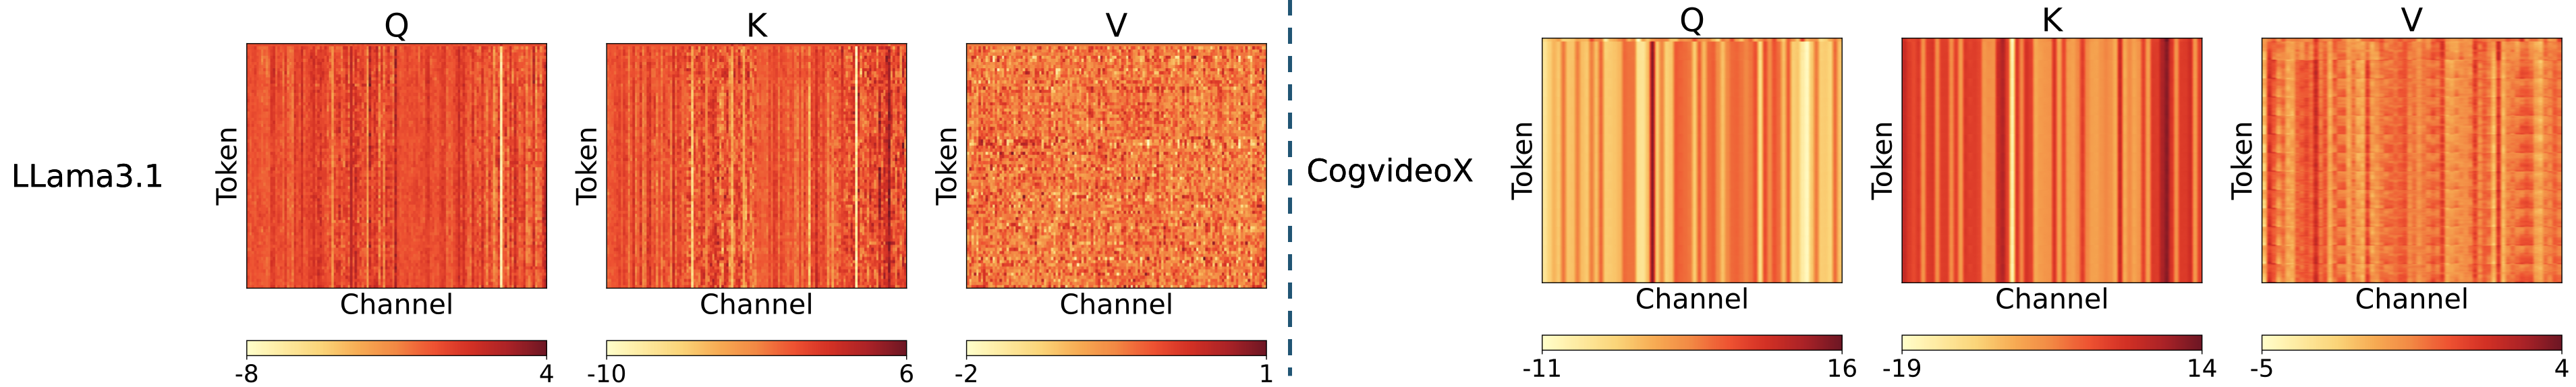
\includegraphics[width=0.999\textwidth]{src/figs/heatmap_onerow.png}
    \vspace{-1.75em}
    \caption{Typical examples of tensors' data distribution in attention.}
    \vspace{-1em}
    \label{fig:smoothqk_heatmaps}
    \end{center}
\end{figure*}


\section{SageAttention2} \label{sec:main_method}
In this section, we introduce SageAttention2, an efficient and accurate quantized attention. The workflow of SageAttention2 is shown in Fig.~\ref{fig:light_overview}. We quantize $Q, K$ to INT4 and $\tilde P, V$ to FP8 to maximize the efficiency and propose several techniques, including $QK$-smoothing, per-thread quantization, and two-level accumulation to preserve the accuracy, which we shall discuss in subsequent subsections. 


\begin{figure}[h!]
    \begin{center}
    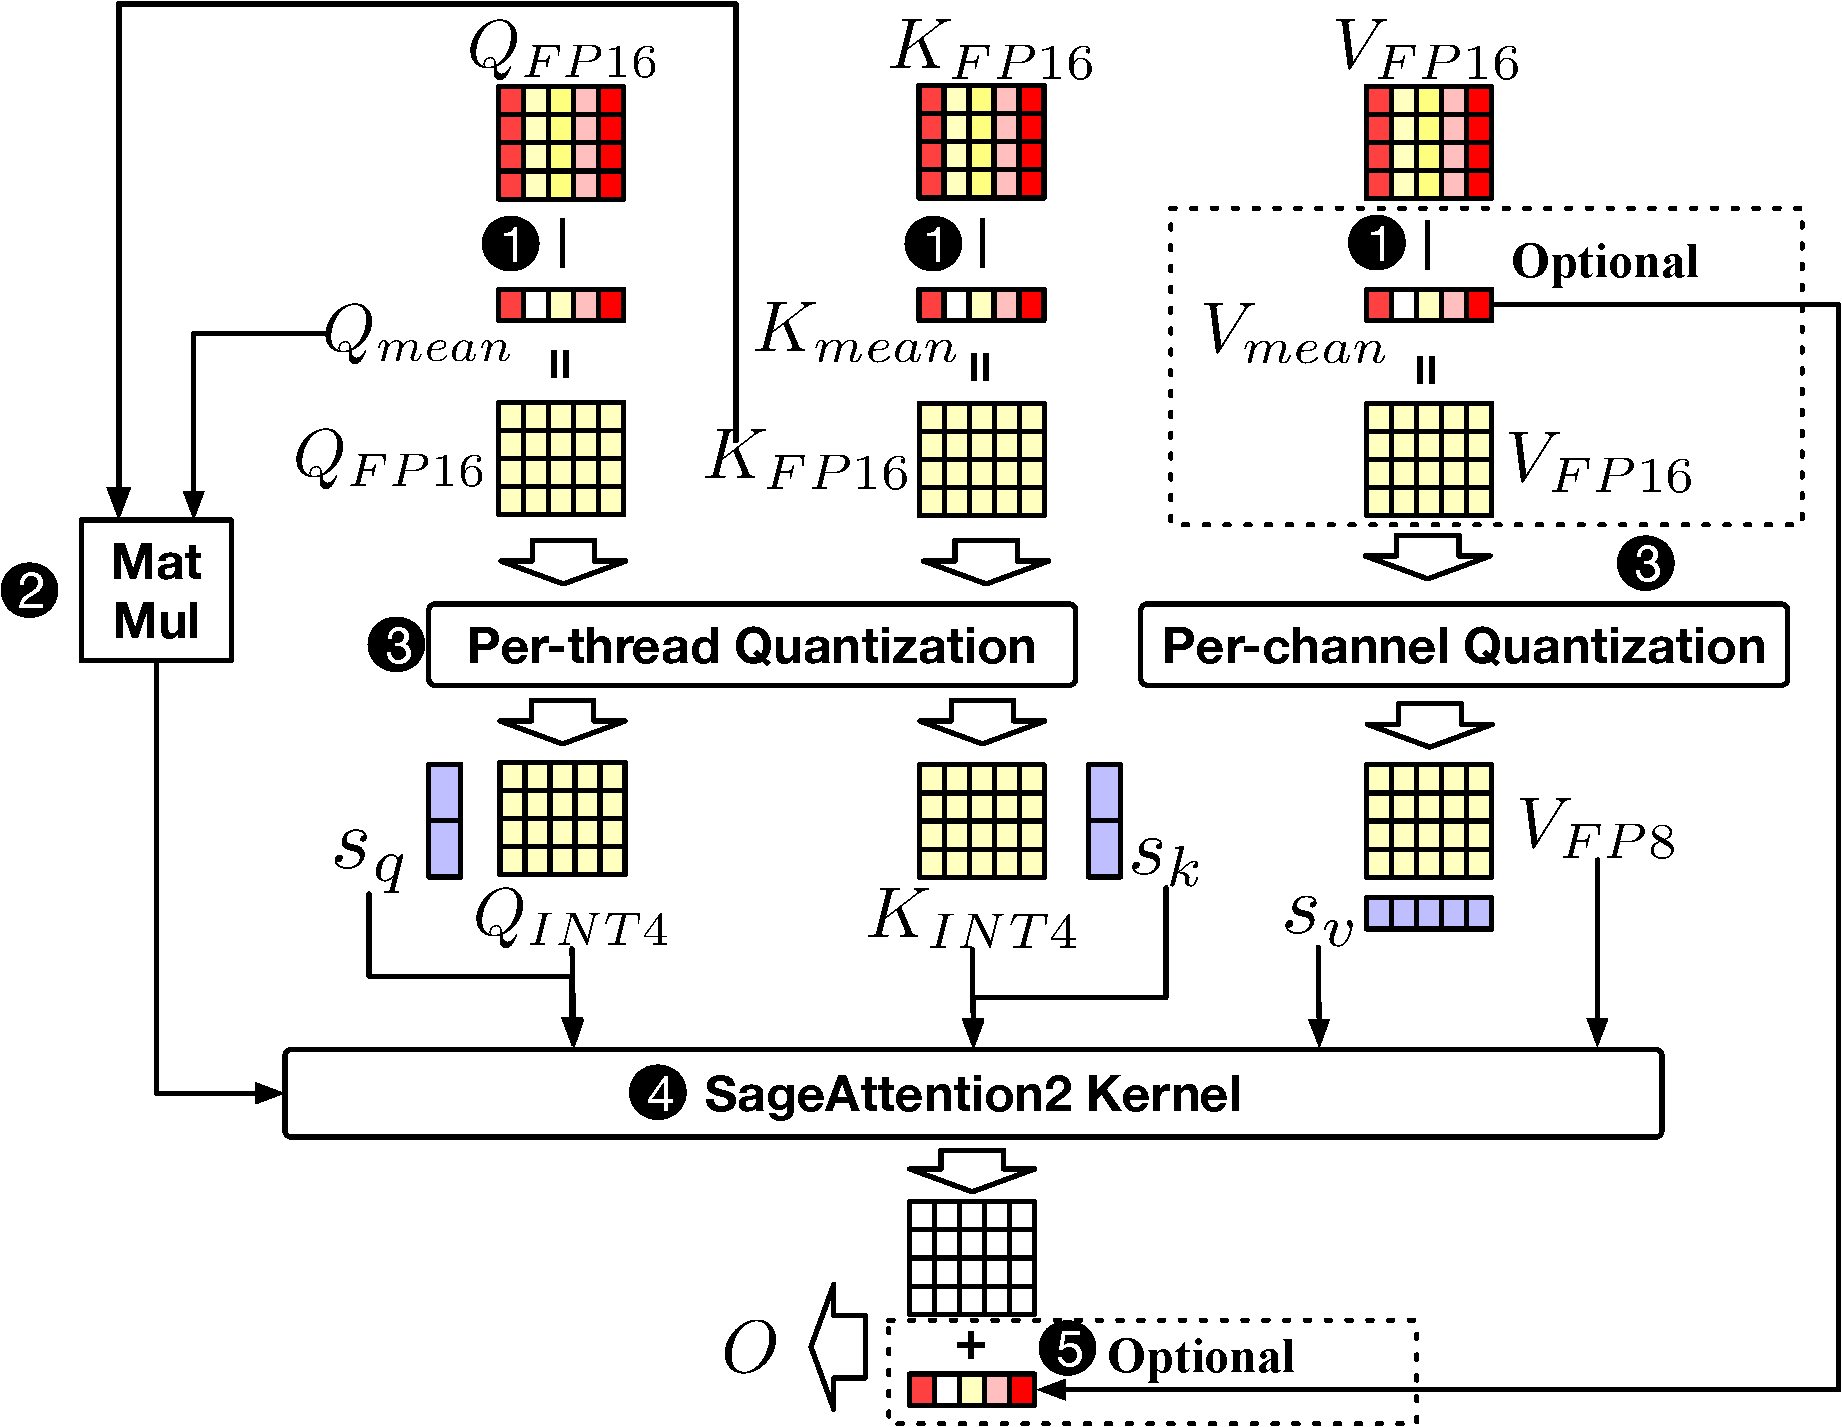
\includegraphics[width=0.48\textwidth]{src/figs/light_framwork.pdf}
    % \vspace{-1.8em}
    \caption{Workflow of \our. \scircled{1} Smooth $Q,K,V$. \scircled{2} A GEMV to obtain $\Delta S$. \scircled{3} Per-thread quantize $Q,K$ and per-channel quantize $V$. \scircled{4} Perform the \our kernel. \scircled{5} Correct the output.}
    \vspace{-1.5em}
    \label{fig:light_overview}
    \end{center}
\end{figure}











\begin{figure*}[h!]
    \begin{center}
    % \vspace{-.36em}
    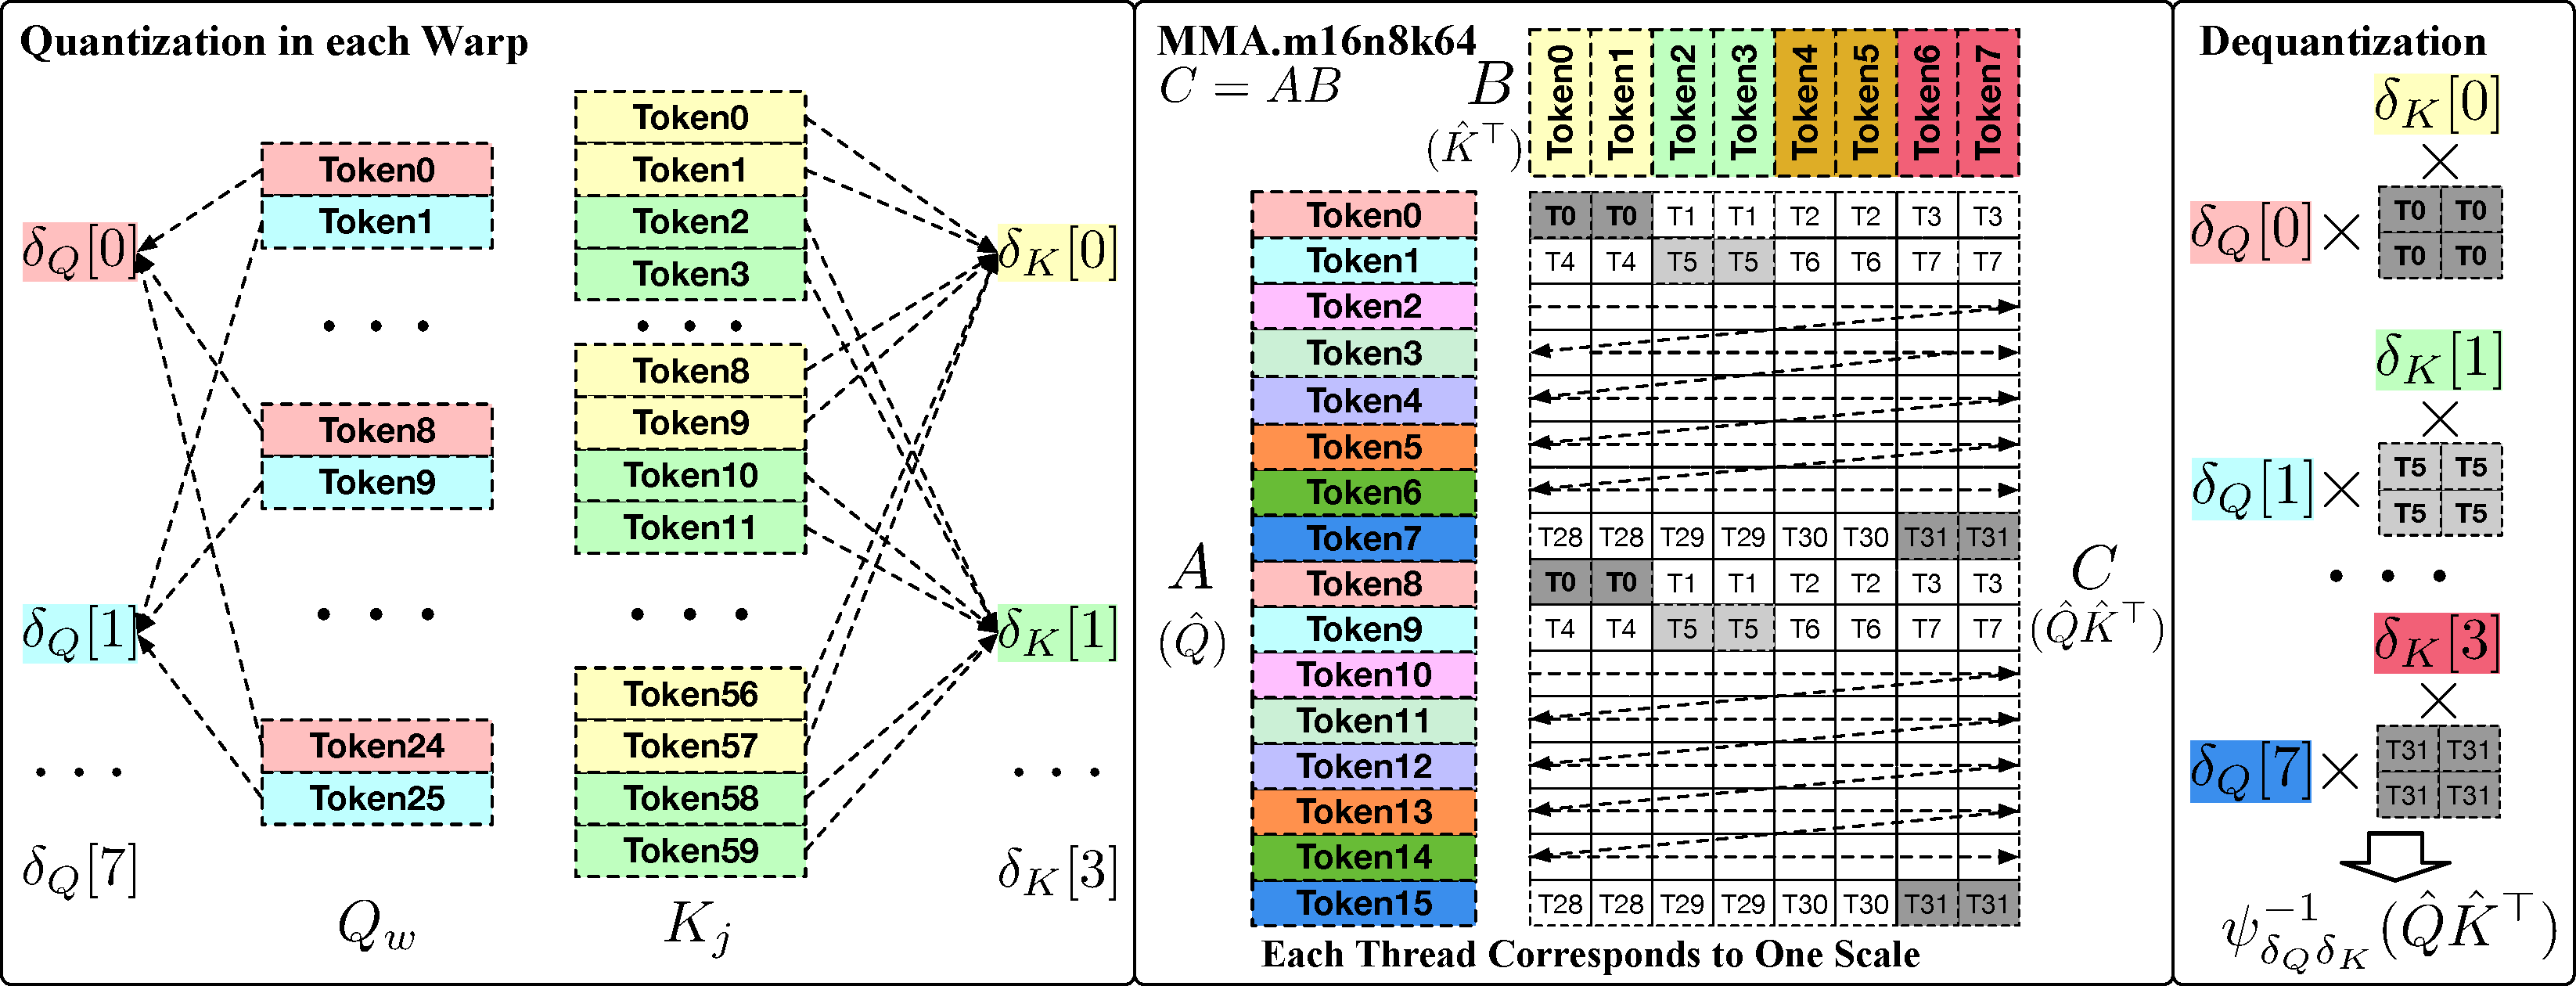
\includegraphics[width=0.999\textwidth]{src/figs/per_thread.pdf}
    \vspace{-1.2em}
    \caption{An example of per-thread quantization. The left figure shows the correspondence between the quantization scales and the tokens in each GPU warp. The right figure shows the correspondence between quantization tokens and GPU threads in a \texttt{MMA.m16n8k64} instruction, showing that each GPU thread only corresponds to one quantization scale in $\delta_Q$ and $\delta_K$ in dequantization.}
    \vspace{-.5em}
    \label{fig:per_thread}
    \end{center}
\end{figure*}



\subsection{Smooth $Q$}
% , i.e., only $2^4-1=15$ values
First, we discuss how to accurately compute $QK^\top$ with INT4. 
The numerical range of INT4 is notably restrictive. This affects quantization due to the presence of \emph{outliers}~\cite{lin2024qserve}. Given the INT4 range [-7, +7], any element will be quantized to zero if it is more than 14 times (0.5 vs 7) smaller than the largest element in the group. Since outliers are much larger than other elements, it is likely that many non-outlier elements are quantized to zero, leading to substantial accuracy degradation.
Therefore, to keep the quantization accurate, we need to keep the largest element small, making the magnitude of elements as uniform as possible. Such technique is called \emph{smoothing}.

Here, we propose a smoothing technique inspired by SageAttention~\cite{2024sageattention}. SageAttention observed that $Q, K$ for all tokens are actually highly similar, with only small variations between different tokens (Fig.~\ref{fig:smoothqk_heatmaps} shows the heatmap distributions of the $Q$, $K$, and $V$ randomly sampled from \llamal~\cite{llama31model} and \cogvideo~\cite{yang2024cogvideox}). 
We propose to smooth $K$ as SageAttention does and further smooth $Q$ by subtracting a common mean of each block:
\begin{align} \label{eqn:smoothing}
\gamma(Q_i) = Q_i - \bar q_i,~~~\gamma(K_j)=K_j-\bar k,
\end{align}
where $\bar q_i=\mean(Q_i), \bar k=\mean(K)$ are  $1\times D$ vectors, the mean is conducted along the token axis, and $\bar q_i, \bar k$ are broadcasted to tokens in a block and a tensor for subtraction. 
% According to our observation, the token-wise variation $\gamma(Q_i), \gamma(K_j)$ are much smaller than $\bar q_i, \bar k$ \haofeng{what does this sentence mean?}. Therefore, it is much more precise to quantize $\gamma(Q_i), \gamma(K_j)$ rather than $Q_i, K_j$. 

With the decomposion, we have $S_{ij}=Q_iK_j^\top=(\bar q_i+\gamma(Q_i))(\bar k+\gamma(K_j))^\top = \bar q_i\bar k^\top + \bar q_i \gamma(K_j)^\top + \gamma(Q_i) \bar k^\top + \gamma(Q_i)\gamma(K_j)^\top =  \gamma(Q_i)\gamma(K_j)^\top + \Delta {S_{ij}} + b$. Here, $\Delta {S_{ij}}=\bar q_i \gamma(K_j)^\top$ is an $1\times N$ vector, and $b=\bar q_i\bar k^\top + \gamma(Q_i) \bar k^\top$ is an $N\times 1$ vector. We do not need to compute $b$  since adding a common bias to an entire row of $S$ does not affect the result after softmax. 
Therefore, we can accelerate $Q_iK_j^\top$ with INT4 by the following two stages:\\
(1) \emph{preprocessing}: smooth $Q, K$ according to  Eq.~(\ref{eqn:smoothing}), apply quantization $(\delta_{Q_i}, \hat Q_i) = \psi_Q(\gamma(Q_i)),(\delta_{K_j}, \hat K_j) = \psi_K(\gamma(K_j))
$, and compute $\Delta{S_{ij}} = \bar q_i\gamma(K_j)^\top$. Smoothing, quantization, and GEMV (general matrix-vector multiplication) for computing $\Delta S$ can be fused into a single kernel, which reads the off-chip $Q$ and $K$ only once.

(2) \emph{attention}: execute the low-precision GEMM, dequantize, and add back the vector $\Delta S$: $S_{ij} = \psi^{-1}_{\delta_{Q_i}\delta_{K_j}}(\hat Q_i \hat K_j^\top) + \Delta S_{ij}$. These operations are all done on chip, and the dequantization and vector addition only add a marginal overhead compared to the expensive \texttt{mma} operation for MM. \\
Importantly, $\gamma(Q_i), \gamma(K_j)$ are quantized rather than $Q_i, K_j$. Since the smoothed matrices are much smaller in magnitude and contain fewer outliers, the quantization accuracy can be significantly improved. A theoretical analysis of the benefit of smoothing is included in Appendix~\ref{sec:smoothing_theoretical}.




\textbf{Remark.} Classical techniques to improve the activation-weight MM, such as per-channel quantization, or SmoothQuant~\cite{xiao2023smoothquant} are not applicable here for the query-key MM in attention. Per-channel quantization cannot be applied to $Q, K$ because the quantization must be conducted along the outer axis (token dimension) of $QK^\top$. On the other hand, both $Q$ and $K$ have significant outliers, so trading the quantization accuracy between them with SmoothQuant cannot work effectively, as shown in Sec.~\ref{sec:exp}. Here, we utilize the unique token similarity pattern in attention to derive a dedicated quantization method for $Q$ and $K$. The previous work SageAttention only smooths $K$, so it is less accurate than our method.


\textbf{Empirical results.}
Fig.~\ref{fig:bucket_usage} in Appendix~\ref{sec:appendix_analysis_exp} shows an example from \cogvideo of the distribution of $\hat Q$ with and without smoothing $Q$. We can find that with smoothing $Q$, the range of INT4 is utilized more uniformly and fully.
Table~\ref{tab:effect_smooth_qk} presents end-to-end metrics for different quantization methods with and without \textit{smoothing Q+K} on \llamal and \cogvideo(2b). The results demonstrate that \textit{smoothing Q+K} offers significant accuracy benefits. Also, Table~\ref{tab:accuracy_compare1} and~\ref{tab:accuracy_compare2} show that the order of effectiveness is \textit{smoothing Q+K} $>$ \textit{smoothing Q} $>$ \textit{smoothing K} $>$ \textit{other baselines}.






\subsection{INT4 Per-thread Quantization} \label{sec:per-warp_quant}
Orthogonal to smoothing, we can mitigate the problem of outliers by refining the quantization granularity so that the number of affected elements by outliers becomes smaller. 
Although per-token quantization offers a detailed level of granularity, it results in significant overhead during dequantization. Specifically, \uline{each GPU thread in per-token quantization must handle multiple quantization scales, leading to a high latency} of the dot product of the quantization scale vectors $\delta_Q$ and $\delta_K$.
SageAttention uses per-block quantization%, which quantizes each block of $Q$ and $K$ for a GPU streaming processor. 
, where each block $Q_i$ ($b_q$ tokens) and $K_i$ ($b_k$ tokens) have a single quantization scale.
% \jianfei{revise this subsection according to previous discussions} \jintao{check}
Such a quantization strategy could achieve an accuracy performance close to per-token quantization and avoid the high dequantization overhead. However, quantizing $Q$ and $K$ to INT4 demands a finer quantization granularity. To address this, we propose \textit{per-thread quantization}, a more precise and granular approach than the \textit{per-block quantizer}, also without the additional overhead of the vector dot product between $\delta_Q$ and $\delta_K$. 

Specifically, each block of $Q$, i.e., $Q_i$, in SageAttention will be split into $c_w$ segments and processed by $c_w$ GPU warps in a GPU streaming processor (SM). We call each segment of $Q_i$ as $Q_w$, and $k_w = K_j$ since $K_j$ is shared among warps. Then, each warp containing 32 threads uses the \texttt{mma.m16n8k64} PTX instruction~\cite{ptx} for the $Q_wK_j^\top$. According to the layout requirement of this instruction, we find that $Q_w[8k+i]$ could share one quantization scale, and $K_j[8k+2i]$ together with $K_j[8k+2i+1]$ could share one quantization scale. Such a quantization method is more fine-grained with no additional overhead. This is because it assigns different GPU threads to distinct quantization groups based on the MMA instruction layout, with each thread performing dequantization only using a single quantization scale value. 
We show an example of per-thread quantization in Fig.~\ref{fig:per_thread}. The detailed formulation is shown in Equation~\ref{equ:per_thread_quant} and Fig.~\ref{fig:tensor_core_layout} (please see Appendix~\ref{sec:per_thread_formulation} for more detail). 

\textbf{Empirical results.}
As shown in Table~\ref{tab:quant_granularities1} and Table~\ref{tab:quant_granularities2}, we compare the average and worst accuracy of INT4 quantization at per-token, per-thread, per-block, and per-tensor granularity using real $Q, K, V$ across all layers of \cogvideo. Results indicate that the accuracy of per-thread quantization is very close to per-token and significantly outperforms other granularities. Moreover, Table~\ref{tab:granularity_speed_ablation} shows that per-thread quantization incurs almost no speed degradation, while per-token quantization introduces noticeable overhead due to the reduced hardware efficiency.




\begin{algorithm*}[htb!]
    \small
    \caption{Implementation of \our.}
    \label{alg:our} 
    % \setlength{\textfloatsep}{-10pt}
    \begin{algorithmic}
    \STATE {\bfseries Input:} {Matrices $Q(\text{FP16}), K(\text{FP16}), V(\text{FP16}) \in \mathbb{R}^{N \times d}$, block size $b_q, b_{kv}$, warp count \jt{$c_w$}.}
    

    \STATE \textbf{Preprocessing:} \jt{$K=K-\mathrm{mean}(K)$}, $~~\jt{(\delta_V, \hat V)} = \jt{\psi_V}(V)$. \annotate{//per-channel.}
    

    \STATE Divide \jt{$Q$} to $T_m = {N}/{b_q}$ blocks \jt{$\{Q_i\}$}; divide \jt{$K$}, and \jt{$V$} to $T_n = {N}/{b_{kv}}$ blocks \jt{$\{K_i\}$}, \jt{$\{V_i\}$};  

    \FOR {$i=1$ {\bfseries to} $T_m$}

      \STATE $\jt{\bar q_i=\mean(Q_i),~~ (\delta_Q, \hat Q_i)} = \jt{\psi_Q(Q_i - \bar q_i)}$ \annotate{//per-thread} ; 

        \FOR {$\textbf{j}$ in [1, $T_n$]} 
            \STATE $\jt{(\delta_K, \hat K_j)} = \jt{\psi_K}(K_j)$ \annotate{//per-thread},   ~~~ \jt{$w = \text{range}(c_w), st = w*c_w$} ; 
            \STATE \jt{$S_{ij}[st:st+c_w] = \psi^{-1}_{\delta_Q\delta_K}(\mathrm{Matmul}(\hat Q_i[st:st+c_w], \hat K_j^\top)) + \text{GEMV}(\bar q_i, K_j^\top)$} ;  \annotate{// Paralleled by $c_w$ warps. The $\psi^{-1}_{\delta_Q\delta_K}$ is illustrated in Fig.~\ref{fig:per_thread}.}

            \STATE $m_{ij} = \mathrm{max}(m_{i,j-1}, \mathrm{rowmax}(S_{ij}))$, $~\widetilde P_{ij} = \mathrm{exp}(S_{ij} - m_{ij})$, $~l_{ij} = e^{m_{i,j-1}-m_{ij}} l_{i,j-1} + \mathrm{rowsum}(\widetilde P_{ij})$ ;

            \STATE $O_{ij}$(FP22) = \jt{$\mathrm{Matmul}((\widetilde P_{ij}*448)\text{.to(FP8.e4m3)}, V_j)$} ;
            
            \STATE \jt{$O_{ij}$(FP32) = $\mathrm{diag}(e^{m_{i,j-1}-m_{ij}}) O_{i,j-1}(FP32) + O_{ij}$(FP22)} ;

        
        \ENDFOR
        \STATE Load \jt{$\delta_{V}$} into an SM ;~~~ $O_i = \mathrm{diag}(l_{i,T_n}) ^{-1} O_{i,T_n}\text{(FP32)}$ \jt{$/ 448 * \delta_{V}$} ;~~~ Write $O_i$ ;  
    \ENDFOR
    
    % \STATE $O = \{O_i\}$
    \STATE \textbf{return} $O = \{O_i\}$
    \end{algorithmic}
    \vspace{-.2em}
\end{algorithm*}


\subsection{FP8 quantization for $\tilde PV$} 
We now turn to the MM $\tilde PV$, where $\tilde P_{ij}=\exp(S_{ij} - m_{ij})$ is the unnormalized quantity according to Eq.~(\ref{eqn:online-softmax}). 
The distribution of $\tilde P$ is unique and differs from other activations. First, we note that $S_{ij} - m_{ij}\le 0$, so $P_{ij}\in [0, 1]$ ($\le$ and $\in$ apply element-wise). We find that $\tilde P$ often consists of many small elements, but their sum is non-negligible (e.g., 5000 elements around $10^{-4}$). In this case, we must represent small elements accurately. INT quantization is unsuitable for this setting, since it distributes the quantization points evenly within the numerical range. SageAttention~\cite{2024sageattention} choose to retain $\tilde P$ and $V$ in FP16, and accelerate the MM by decreasing the accumulator precision. However, this strategy is only effective on very few GPUs.


We propose to quantize $\widetilde P, V$ to FP8 with 4 exponent bits and 3 mantissa bits (E4M3). The numerical range of E4M3 is $[-448, +448]$. We quantize $P$ with a static scale: $\delta_P=\frac{1}{448}$ since the original $P$ elements are already in $[0, 1]$. 
We quantize $V$ per-channel to address the channel-wise outliers shown in Fig.~\ref{fig:smoothqk_heatmaps}. 
Empirical results in Table~\ref{tab:quant_data_type1} and Table~\ref{tab:quant_data_type2} show the average and worst accuracy of different data types used for $\widetilde P, V$  across all layers of \cogvideo. The accumulator is always 32-bit. We can see that the accuracy of E4M3 is very close to that of FP16 and superior to  E5M2 and INT8.
Most modern GPUs have tensor cores that support FP8 Matmul operations, which are twice as fast as those using FP16. 


\subsection{FP32 MMA Buffer for FP22 Accumulator}
While FP8 quantization for $\tilde PV$ above is theoretically accurate in simulation, we observe that the actual CUDA implementation suffers a consistent accuracy degradation. After narrowing down the problem, we find that the accumulator for the \texttt{mma(f32f8f8f32)} instruction on the Ada and Hopper architecture is actually FP22, specifically with 1 sign bit, 8 exponent bits, and 13 mantissa bits. Specifically, for \texttt{mma(f32f8f8f32)} instruction $C = AB + D$, where $A, B$ are FP8 matrices and $C, D$ are FP32 matrices, we initialize the $A, B$ to zero and vary $D$ to test the data type of the accumulator. 
When $D$ is initialized with 1 sign bit, 8 exponent bits, and 13 mantissa bits, the value of $C$ exactly matches $D$. However, when $D$ is initialized with more than 13 mantissa bits, the value of $C$ is equal to $D$ with its least significant 10 mantissa bits zeroed out (i.e., truncated).
Consequently, matrix multiplication of $\widetilde 
PV$, quantized to FP8, incurs a certain degree of accuracy loss compared to using an FP32 accumulator. 

To mitigate this accuracy loss, we adopt a two-level accumulation strategy, which uses an FP32 buffer to accumulate the values of $\widetilde{P}_{ij} V_j$ in FP22. Specifically, we rewrite Eq.~(\ref{eqn:online-softmax}) as 
$
R_{ij} = \widetilde P_{ij} V_j,O_{ij}=\diag{\exp(m_{i,j-1}-m_{ij})} O_{i,j-1} + R_{ij} 
$. Here, two sets of accumulators $R_{ij}$ and $O_{ij}$ are maintained in the register. $R_{ij}$ is computed with the \texttt{mma(f32f8f8f32)} instruction, providing 22 effective bits, which is sufficient since we only accumulate over a small number of $b_k$ tokens (e.g., $b_k=64$). Then, $R_{ij}$ is accumulated to $O_{ij}$ in the high FP32 precision.

\textbf{Remark.} 
The two-level accumulation strategy is also implemented in CUTLASS~\cite{cutlass} and DeepGemm~\cite{deepseekai2024deepseekv3technicalreport} for computing weight-activation products in linear layers. To the best of our knowledge, we are the first to discover and investigate the effect of the FP22 accumulator and implement the two-level accumulation for \emph{attention}.








\textbf{Optional smooth V technique.}  
We also figure out another way to mitigate the accuracy loss due to the FP22 accumulator when $V$ possesses channel-wise biases: $\overrightarrow{V_m} = \mathrm{mean}(V, \text{axis}=0), V = V - \overrightarrow{V_m}$.
Furthermore, to maintain the correctness of the attention computation, it is only necessary to add $\overrightarrow{V_m}$ to the final calculation of $O$: $O = O + \overrightarrow{V_m}$. This is because the sum of each row of the $\widetilde P$ matrix equals 1, so $\widetilde P\overrightarrow{V_m} = \overrightarrow{V_m}$.





\textbf{Remark.} For details on smoothing V, see Appendix~\ref{sec:appendix_smooth_v}. This technique is optional and not employed in our main experiments, as it provides significant benefits only when $V$ exhibits channel-wise bias, which are absent in some models, such as \llamal (see Fig.~\ref{fig:smoothqk_heatmaps}). 
